\documentclass{article}
\usepackage[utf8]{inputenc}
\usepackage{tikz}
\usetikzlibrary{positioning,arrows,calc,shapes}
\tikzset{
    on grid,
    node distance=3cm,
    auto,
    process/.style = {
        draw,
        shape=rectangle,
        minimum height=3.5em,
        minimum width=3em,
        line width=1pt
    },
    simulation/.style = {
        draw,
        shape=rectangle,
        minimum height=3em,
        minimum width=3em,
        line width=1pt,
        rounded corners
    },
    module/.style = {
        draw,
        shape=rectangle,
        minimum height=5em,
        minimum width=5em,
        line width=1pt,
        dashed
    },
    multiplexer/.style={
        draw,
        shape=trapezium,
        shape border uses incircle,
        shape border rotate=270,
        minimum size=20pt
    },
    ram/.style = {
        draw,
        shape=rectangle,
        minimum height=3em,
        minimum width=3em,
        line width=0.5pt,
        double
    },
    >=latex',
}


\begin{document}

\section{Modules}

% -------------------------------------------------
% Acceleration 1.1

\begin{figure}
    \centering
    \scalebox{0.7}{
        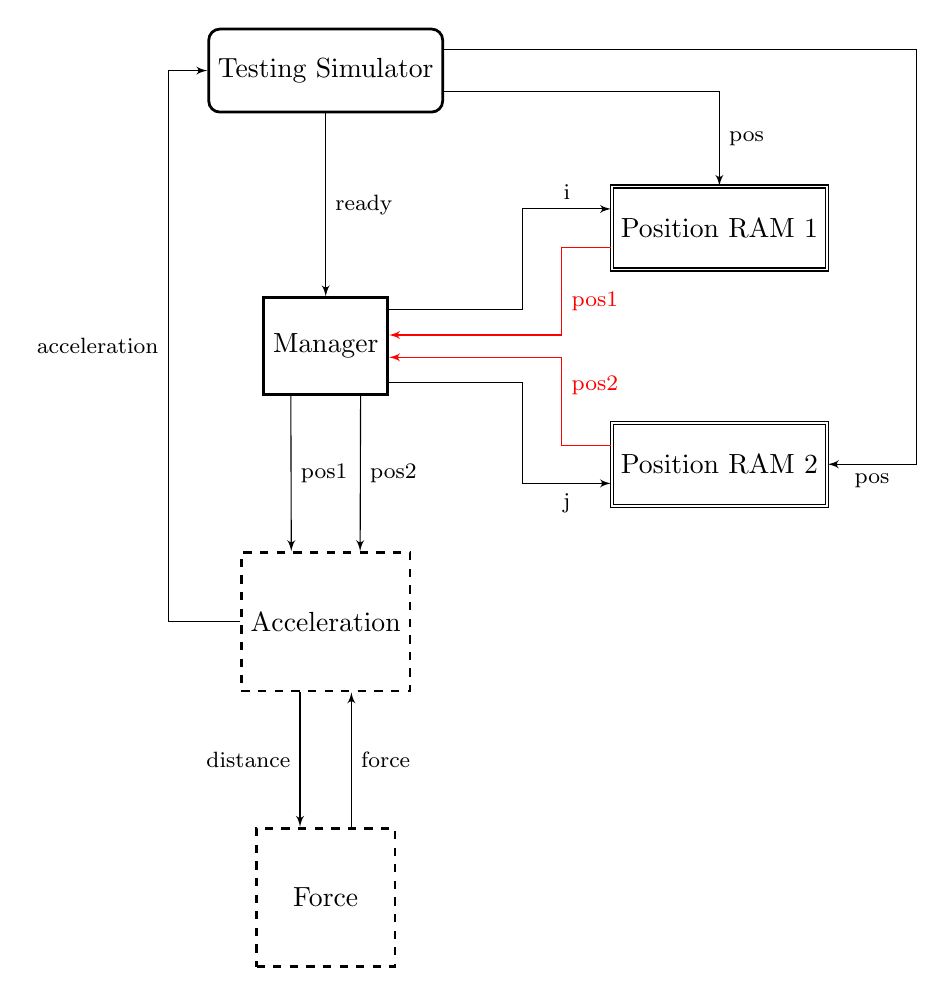
\begin{tikzpicture}
            \node[ram] (posram1) at (5,2) {Position RAM 1};
            \node[ram] (posram2) at (5,-1) {Position RAM 2};
            \node[process] (manager) at (0,.5) {Manager};
            \node[simulation] (testsim) at (0,4) {Testing Simulator};
            \node[module] (acceleration) at (0,-3) {Acceleration};
            \node[module] (force) at (0,-6.5) {Force};

            \path[draw, ->] (testsim.350) -| (posram1.90) node [near end] {\footnotesize pos};
            \path[draw, ->] (testsim.10) -| (7.5,-1) |- (posram2.0) node [near end] {\footnotesize pos};

            \path[draw, ->] (manager.30) -| (2.5,2) |- (posram1.170) node [near end] {\footnotesize i};
            \path[draw, ->] (manager.330) -| (2.5,0) |- (posram2.190) node [below,near end] {\footnotesize j};

            \path[draw, ->, red] (posram1.190) -| (3,1.5) |- (manager.10) node [near start] {\footnotesize pos1};
            \path[draw, ->, red] (posram2.170) -| (3,0) |- (manager.350) node [right,pos=0] {\footnotesize pos2};

            \path[draw, ->] (testsim.270) -- (manager.90) node [midway] {\footnotesize ready};

            \path[draw, ->] (manager.235) -- (acceleration.116) node [midway] {\footnotesize pos1};
            \path[draw, ->] (manager.305) -- (acceleration.64) node [midway] {\footnotesize pos2};

            \path[draw, ->] (acceleration.250) -- (force.110) node [midway, left] {\footnotesize distance};
            \path[draw, ->] (force.70) -- (acceleration.290) node [midway, right] {\footnotesize force};

            \path[draw, ->] (acceleration.180) -| (-2, -3) |- (testsim.180) node [near start] {\footnotesize acceleration};

        \end{tikzpicture}
    }
    \caption{Acceleration module 1.1}
\end{figure}

% -------------------------------------------------
% Acceleration 1.2

\begin{figure}
    \centering
    \scalebox{0.7}{
        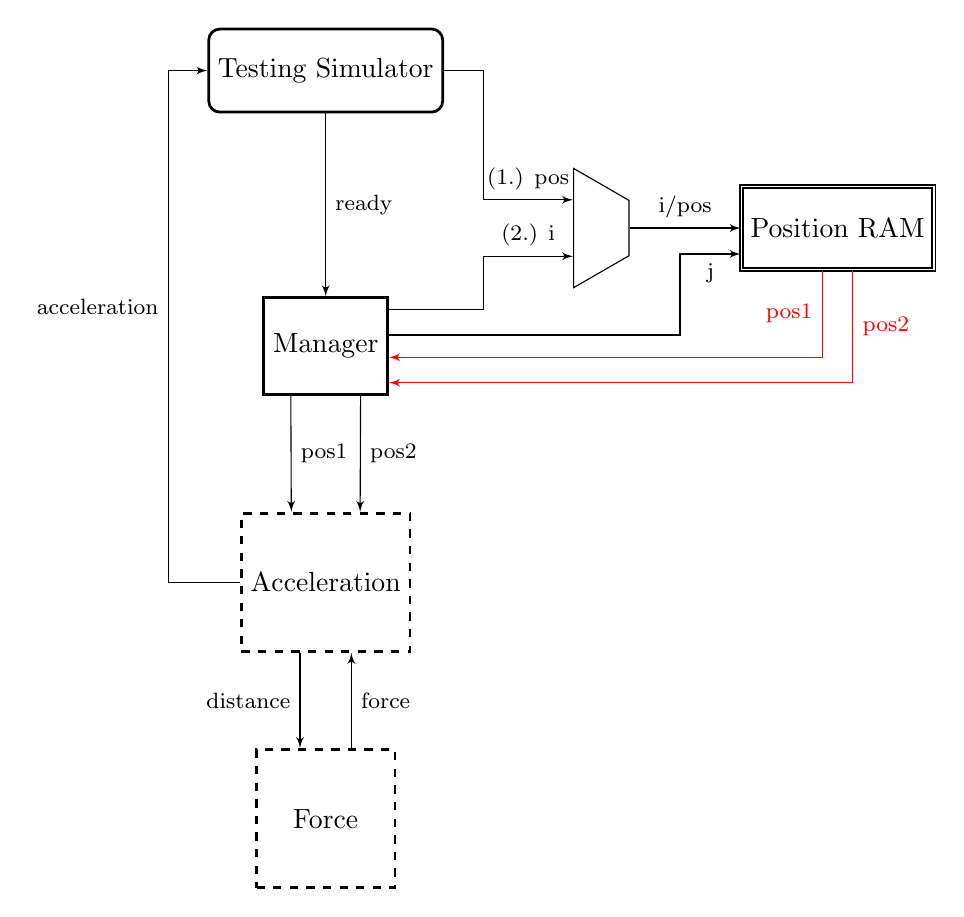
\begin{tikzpicture}
            \node[ram] (posram) at (6.5,1) {Position RAM};
            \node[multiplexer] (mux) at (3.5,1) {};
            \node[process] (manager) at (0,-.5) {Manager};
            \node[simulation] (testsim) at (0,3) {Testing Simulator};
            \node[module] (acceleration) at (0,-3.5) {Acceleration};
            \node[module] (force) at (0,-6.5) {Force};

            \path[draw, ->] (testsim.0) -| (2,3) |- (mux.north west) node [near end] {\footnotesize (1.) pos};
            \path[draw, ->] (manager.30) -| (2,0) |- (mux.south west) node [near end] {\footnotesize (2.) i};

            \path[draw, ->] (manager.10) -| (4.5,0) |- (posram.195) node [near end, below] {\footnotesize j};

            \path[draw, ->, red] (posram.250) |-  (manager.350) node [near start, left] {\footnotesize pos1};
            \path[draw, ->, red] (posram.290) |-  (manager.330) node [near start] {\footnotesize pos2};

            \path[draw, ->] (mux.top side) -- (posram.180) node [midway] {\footnotesize i/pos};


            \path[draw, ->] (testsim.270) -- (manager.90) node [midway] {\footnotesize ready};

            \path[draw, ->] (manager.235) -- (acceleration.116) node [midway] {\footnotesize pos1};
            \path[draw, ->] (manager.305) -- (acceleration.64) node [midway] {\footnotesize pos2};

            \path[draw, ->] (acceleration.250) -- (force.110) node [midway, left] {\footnotesize distance};
            \path[draw, ->] (force.70) -- (acceleration.290) node [midway, right] {\footnotesize force};

            \path[draw, ->] (acceleration.180) -| (-2, -3) |- (testsim.180) node [near start] {\footnotesize acceleration};

        \end{tikzpicture}
    }
    \caption{Acceleration module 1.2}
\end{figure}

% -------------------------------------------------
% Cache 1.1

\begin{figure}
    \centering
    \scalebox{0.8}{
        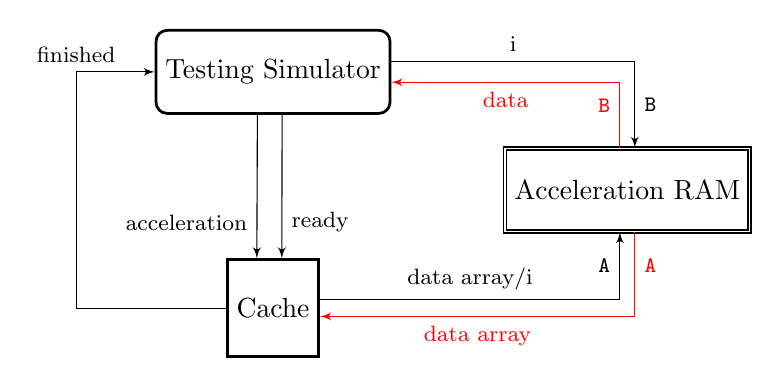
\begin{tikzpicture}
            \node[ram] (accram) at (4.5,-1.5) {Acceleration RAM};
            \node[simulation] (testsim) at (0,0) {Testing Simulator};
            \node[process] (cache) at (0,-3) {Cache};

            \path[draw, ->] (testsim.250) -- (cache.108) node [near end, left] {\footnotesize acceleration};
            \path[draw, ->] (testsim.282) -- (cache.80) node [near end] {\footnotesize ready};
            \path[draw, ->] (cache.10) -| node [near start] {\footnotesize data array/i} (accram.260) node [near end] {\footnotesize \texttt{A}};
            \path[draw, ->, red] (accram.280) |- node [pos=0.2] {\footnotesize \texttt{A}} (cache.350) node [near end] {\footnotesize data array};
            \path[draw, ->] (testsim.5) -| node [near start] {\footnotesize i} (accram.80) node [near end] {\footnotesize \texttt{B}};
            \path[draw, ->, red] (accram.100) |- node [pos=0.32] {\footnotesize \texttt{B}} (testsim.355) node [near end] {\footnotesize data};

            \path[draw, ->] (cache.180) -| (-2.5,-3) |- (testsim.180) node [midway] {\footnotesize finished};

        \end{tikzpicture}
    }
    \caption{Cache module 1.1}
\end{figure}

% -------------------------------------------------
% Velocity-(/position-)update module 1.1

\begin{figure}
    \centering
    \scalebox{0.8}{
        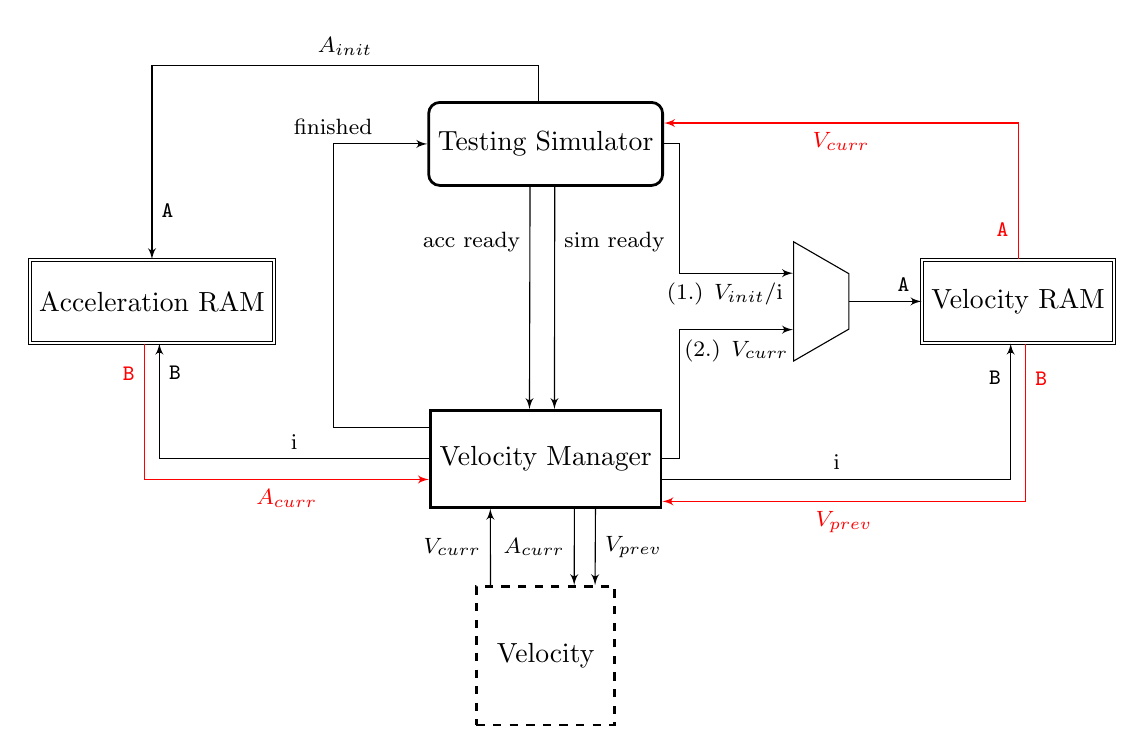
\begin{tikzpicture}
            \node[ram] (accram) at (-5,-2) {Acceleration RAM};
            \node[ram] (veloram) at (6,-2) {Velocity RAM};
            \node[simulation] (testsim) at (0,0) {Testing Simulator};
            \node[process] (manager) at (0,-4) {Velocity Manager};
            \node[module] (velocity) at (0,-6.5) {Velocity};
            \node[multiplexer, shape border rotate=270] (mux) at (3.5,-2) {};

            \path[draw, ->] (testsim.250) -- (manager.108) node [near start, left] {\footnotesize acc ready};
            \path[draw, ->] (testsim.282) -- (manager.80) node [near start] {\footnotesize sim ready};
            \path[draw, ->] (velocity.128) -- (manager.222) node [midway] {\footnotesize $V_{curr}$};
            \path[draw, ->] (manager.300) -- (velocity.68) node [midway, left] {\footnotesize $A_{curr}$};
            \path[draw, ->] (manager.315) -- (velocity.55) node [midway] {\footnotesize $V_{prev}$};

            \path[draw, ->] (manager.350) -| node [near start] {\footnotesize i} (veloram.260) node [very near end] {\footnotesize \texttt{B}};
            \path[draw, ->, red] (veloram.280) |- node [pos=0.11] {\footnotesize \texttt{B}} (manager.340) node [near end] {\footnotesize $V_{prev}$};

            \path[draw, ->] (manager.180) -| node [near start, above] {\footnotesize i} (accram.280) node [very near end, right] {\footnotesize \texttt{B}};
            \path[draw, ->, red] (accram.260) |- node [pos=0.11, left] {\footnotesize \texttt{B}} (manager.190) node [near end, below] {\footnotesize $A_{curr}$};
            \path[draw, ->] (manager.0) -| (1.7,-3) |- (mux.south west) node [near end, below] {\footnotesize (2.) $V_{curr}$};
            \path[draw, ->] (testsim.0) -| (1.7,-1) |- (mux.north west) node [pos=0.7, below] {\footnotesize (1.) $V_{init}$/i};

            \path[draw, ->] (mux.east) -- (veloram.180) node [near end] {\footnotesize \texttt{A}};
            \path[draw, ->] (testsim.100) |- (-5, 1) node [near end, above] {\footnotesize $A_{init}$} -| (accram.90) node [very near end] {\footnotesize \texttt{A}};

              \path[draw, ->, red] (veloram.90) |- node [pos=0.11] {\footnotesize \texttt{A}} (testsim.10) node [near end] {\footnotesize $V_{curr}$};

            \path[draw, ->] (manager.165) -| (-2.7,-3) |- (testsim.180) node [midway] {\footnotesize finished};

        \end{tikzpicture}
    }
    \caption{Velocity-(/Position)-update module 1.1}
\end{figure}


% -------------------------------------------------
% LJ complete circuit

\begin{figure}
    \centering
    \scalebox{0.6}{
        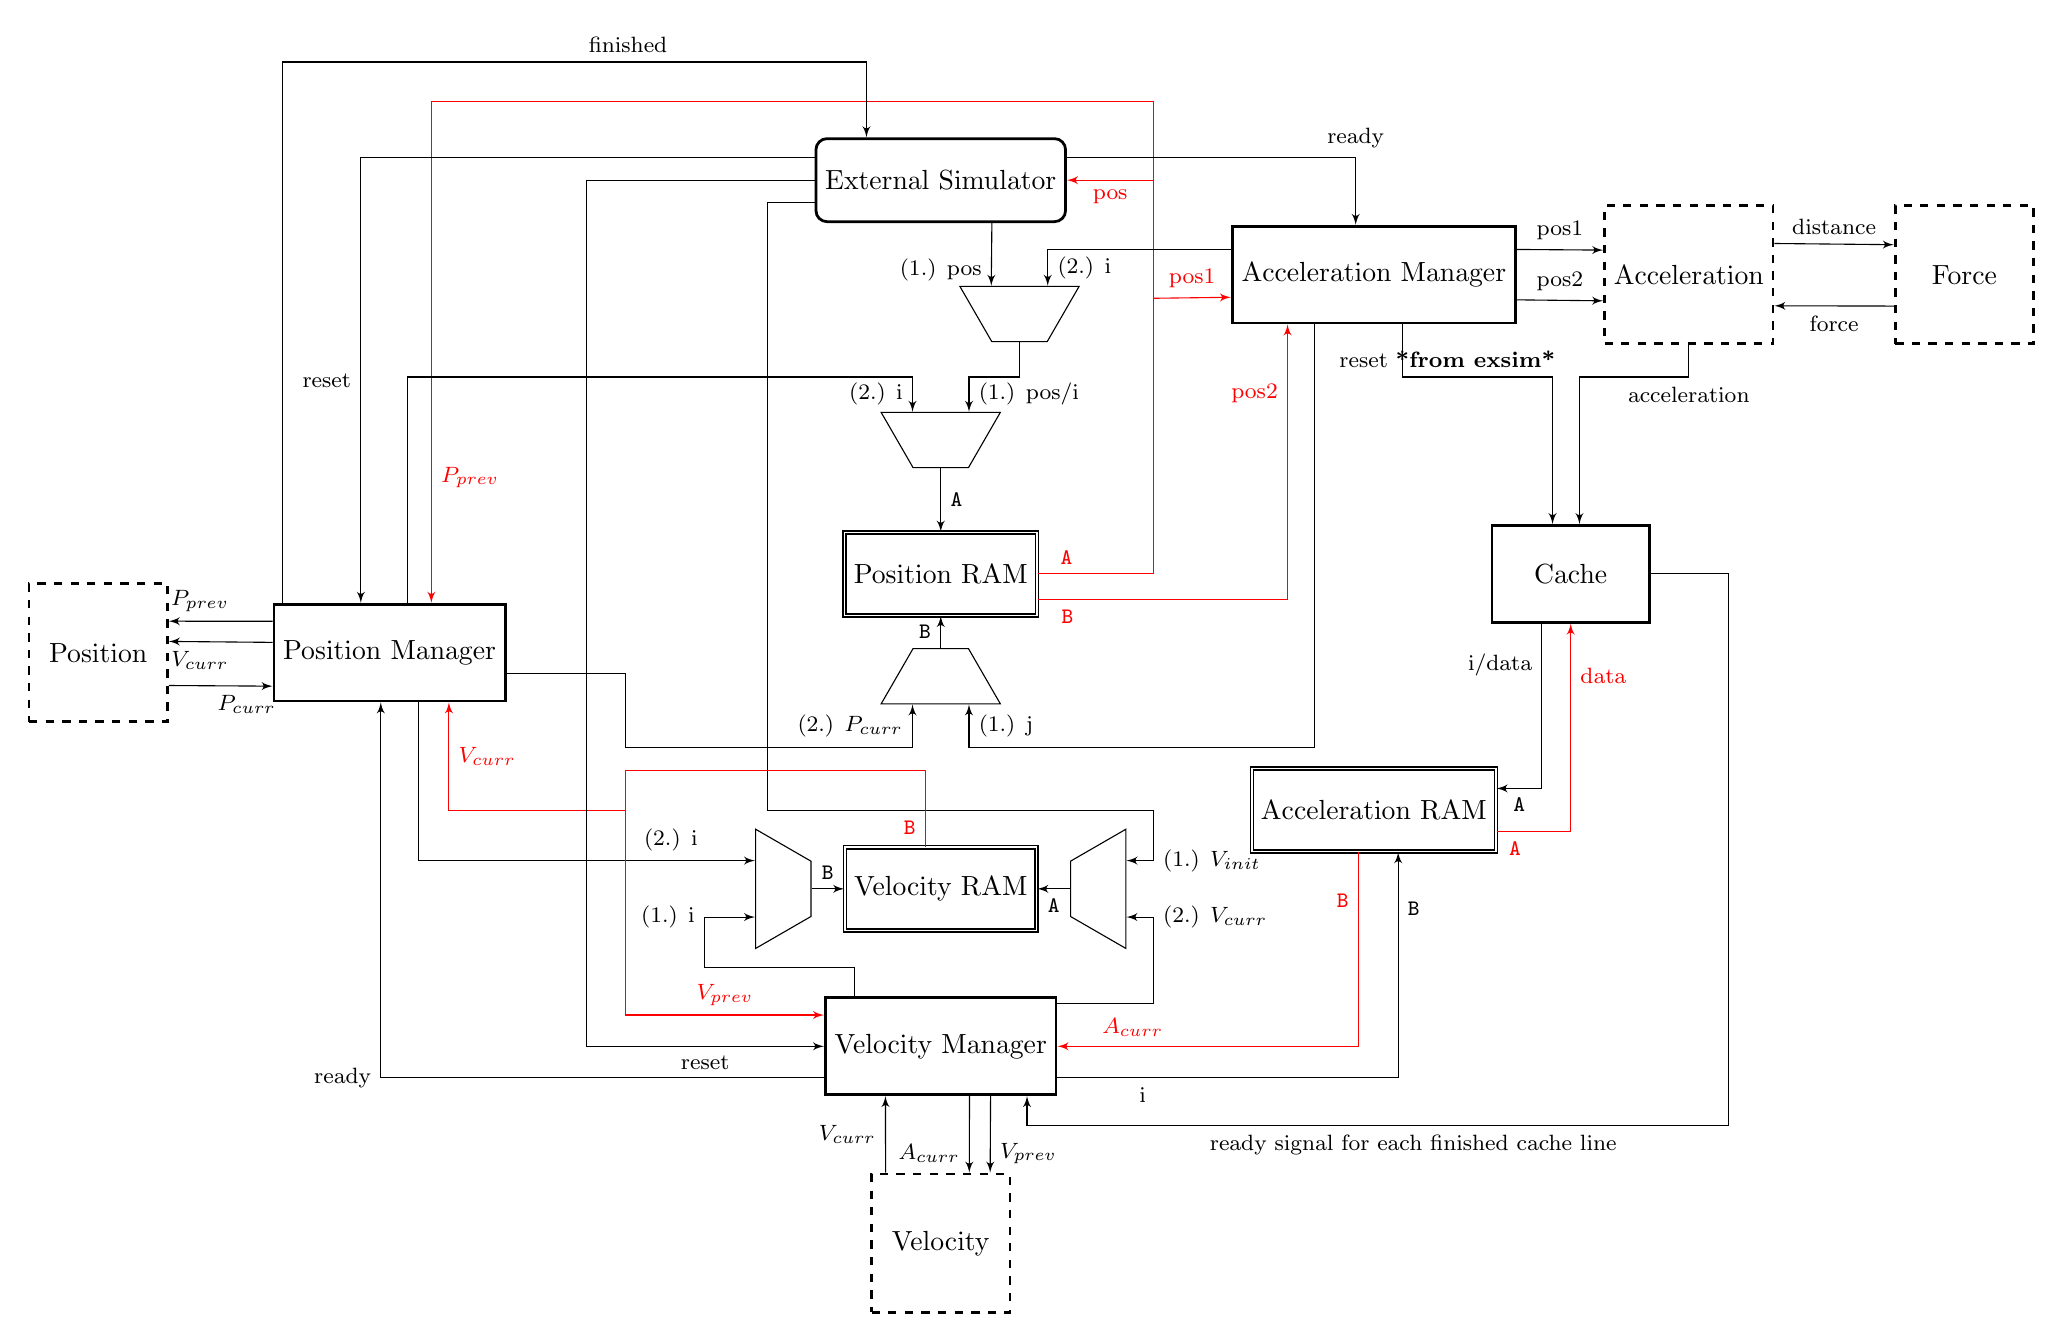
\begin{tikzpicture}
            \node[simulation] (exsim) at (0,0) {External Simulator};
            \node[ram] (posram) at (0,-5) {Position RAM};
            \node[ram] (accram) at (5.5,-8) {Acceleration RAM};
            \node[ram] (veloram) at (0,-9) {Velocity RAM};

            \node[multiplexer, shape border rotate=180] (mux1) at (1,-1.7) {};
            \node[multiplexer, shape border rotate=180] (mux2) at (0,-3.3) {};
            \node[multiplexer, shape border rotate=0] (mux3) at (0,-6.3) {};
            \node[multiplexer, shape border rotate=90] (mux4) at (2,-9) {};
            \node[multiplexer, shape border rotate=270] (mux5) at (-2,-9) {};
            \node[process] (accmanager) at (5.5,-1.2) {Acceleration Manager};
            \node[process, minimum width=2cm] (cache) at (8,-5) {Cache};
            \node[process] (velmanager) at (0,-11) {Velocity Manager};
            \node[process] (posmanager) at (-7,-6) {Position Manager};
            \node[module] (acceleration) at (9.5,-1.2) {Acceleration};
            \node[module] (force) at (13,-1.2) {Force};
            \node[module] (velocity) at (0,-13.5) {Velocity};
            \node[module] (position) at (-10.7,-6) {Position};

            \path[draw, ->] (exsim.320) -- (mux1.north west) node [left, near end] {\footnotesize (1.) pos};
            \path[draw, ->] (mux1.south) |- (1,-2.5) -| (mux2.north east) node [near end] {\footnotesize (1.) pos/i};
            \path[draw, ->] (mux2.south) -| (posram.90) node [near end] {\footnotesize \texttt{A}};


            \path[draw, ->, red] (posram.0) -| node [very near start] {\footnotesize \texttt{A}} (2.7,-5) |- (exsim.0) node [near end] {\footnotesize pos};

            \path[draw, ->, red] (2.7,-0) |- (2.7,1) -| (posmanager.50) node [very near end] {\footnotesize $P_{prev}$};
            \path[draw, ->, red] (2.7,-1.5) -- (accmanager.189) node [midway] {\footnotesize pos1};

            \path[draw, ->, red] (posram.345) -| node [pos=0.06, below] {\footnotesize \texttt{B}} (accmanager.210) node [very near end, left] {\footnotesize pos2};


            \path[draw, ->] (accmanager.170) -| (mux1.north east) node [near end] {\footnotesize (2.) i};
            \path[draw, ->] (accmanager.220) |- (4.5,-7.2) -| (mux3.south east) node [near end, right] {\footnotesize (1.) j};

            \path[draw, ->] (exsim.10) -| (accmanager.110) node [midway, above] {\footnotesize ready};

            \path[draw, ->] (accmanager.300) |- (7,-2.5) node [near end] {\footnotesize reset \textbf{*from exsim*}} -| (cache.110) ;

            \path[draw, ->] (acceleration.270) |- node [midway] {\footnotesize acceleration} (9,-2.5) -| (cache.80) ;

            \path[draw, ->] (cache.240) |- node [very near start, left] {\footnotesize i/data} (accram.10) node [near end] {\footnotesize \texttt{A}};
            \path[draw, ->, red] (accram.350) -| node [very near start, below] {\footnotesize \texttt{A}} (cache.270) node [very near end, right] {\footnotesize data};

            \path[draw, ->] (accmanager.10) -- (acceleration.164) node [midway] {\footnotesize pos1};
            \path[draw, ->] (accmanager.350) -- (acceleration.197) node [midway] {\footnotesize pos2};

            \path[draw, ->] (acceleration.20) -- (force.157) node [midway] {\footnotesize distance};
            \path[draw, ->] (force.204) -- (acceleration.340) node [midway] {\footnotesize force};

            \path[draw, ->, red] (accram.250) |- node [very near start, left] {\footnotesize \texttt{B}} (velmanager.0) node [very near end, above] {\footnotesize $A_{curr}$};
            \path[draw, ->] (velmanager.345) -| node [very near start, below] {\footnotesize i} (accram.300) node [very near end, right] {\footnotesize \texttt{B}};

            \path[draw, ->] (cache.0) -| (10, -5) |- node [near end] {\footnotesize ready signal for each finished cache line} (2,-12) -| (velmanager.330);

            \path[draw, ->] (velmanager.300) -- (velocity.68) node [near end, left] {\footnotesize $A_{curr}$};
            \path[draw, ->] (velmanager.315) -- (velocity.55) node [near end] {\footnotesize $V_{prev}$};
            \path[draw, ->] (velocity.128) -- (velmanager.222) node [midway] {\footnotesize $V_{curr}$};


            \path[draw, ->] (mux4.west) -- (veloram.0) node [midway] {\footnotesize \texttt{A}};

            \path[draw, ->] (velmanager.20) -| (2.7,-10) |- node [midway, right] {\footnotesize (2.) $V_{curr}$} (mux4.south east);
            \path[draw, ->] (exsim.190) -| (-2.2,-8) -| (2.7,-8) |- node [midway, right] {\footnotesize (1.) $V_{init}$} (mux4.north east);

            \path[draw, ->] (mux5.east) -- (veloram.180) node [midway] {\footnotesize \texttt{B}};

            \path[draw, ->] (velmanager.150) |- (-3,-10) |- node [midway, left] {\footnotesize (1.) i} (mux5.south west);
            \path[draw, ->] (posmanager.300) |- node [very near end] {\footnotesize (2.) i} (mux5.north west);

            \path[draw, ->, red] (veloram.110) |- node [very near start] {\footnotesize \texttt{B}} (-3, -7.5) -| (-4,-8) |- (velmanager.165) node [near end] {\footnotesize $V_{prev}$};

            \path[draw, ->, red] (-4,-8) -| (posmanager.320) node [near end, right] {\footnotesize $V_{curr}$};

            \path[draw, ->] (exsim.180) -| (-4.5,-11) |- (velmanager.180) node [near end, below] {\footnotesize reset};

            \path[draw, ->] (posmanager.165) -- (position.24) node [pos=0.7, above] {\footnotesize $P_{prev}$};
            \path[draw, ->] (posmanager.175) -- (position.9) node [pos=0.7] {\footnotesize $V_{curr}$};
            \path[draw, ->] (position.335) -- (posmanager.196) node [near end, below] {\footnotesize $P_{curr}$};

            \path[draw, ->] (velmanager.195) -| (posmanager.260) node [midway] {\footnotesize ready};


            \path[draw, ->] (mux3.north) -- (posram.270) node [midway] {\footnotesize \texttt{B}};

            \path[draw, ->] (posmanager.350) -| (-4,-6.5) |- (-4,-7.2) -| (mux3.south west) node [near end, left] {\footnotesize (2.) $P_{curr}$};

            \path[draw, ->] (posmanager.70) |- (-4,-2.5) -| (mux2.north west) node [near end, left] {\footnotesize (2.) i};

            \path[draw, ->] (exsim.170) -| (posmanager.120) node [near end, left] {\footnotesize reset};

            \path[draw, ->] (posmanager.155) |- (-7,1.5) -| node [near start] {\footnotesize finished} (exsim.150) ;
        \end{tikzpicture}
    }
    \caption{Full LJ circuit}
\end{figure}

% -------------------------------------------------
% Cache 1.1


\section{Function wrappers}
$$\left(48 \cdot \epsilon \cdot \left( \frac{\sigma^{12}}{r^{14}}\right)\right) - \left(24 \cdot \epsilon \cdot\left(\frac{\sigma^6}{r^8} \right) \right)$$
\begin{figure}
    \centering
    \scalebox{0.8}{
        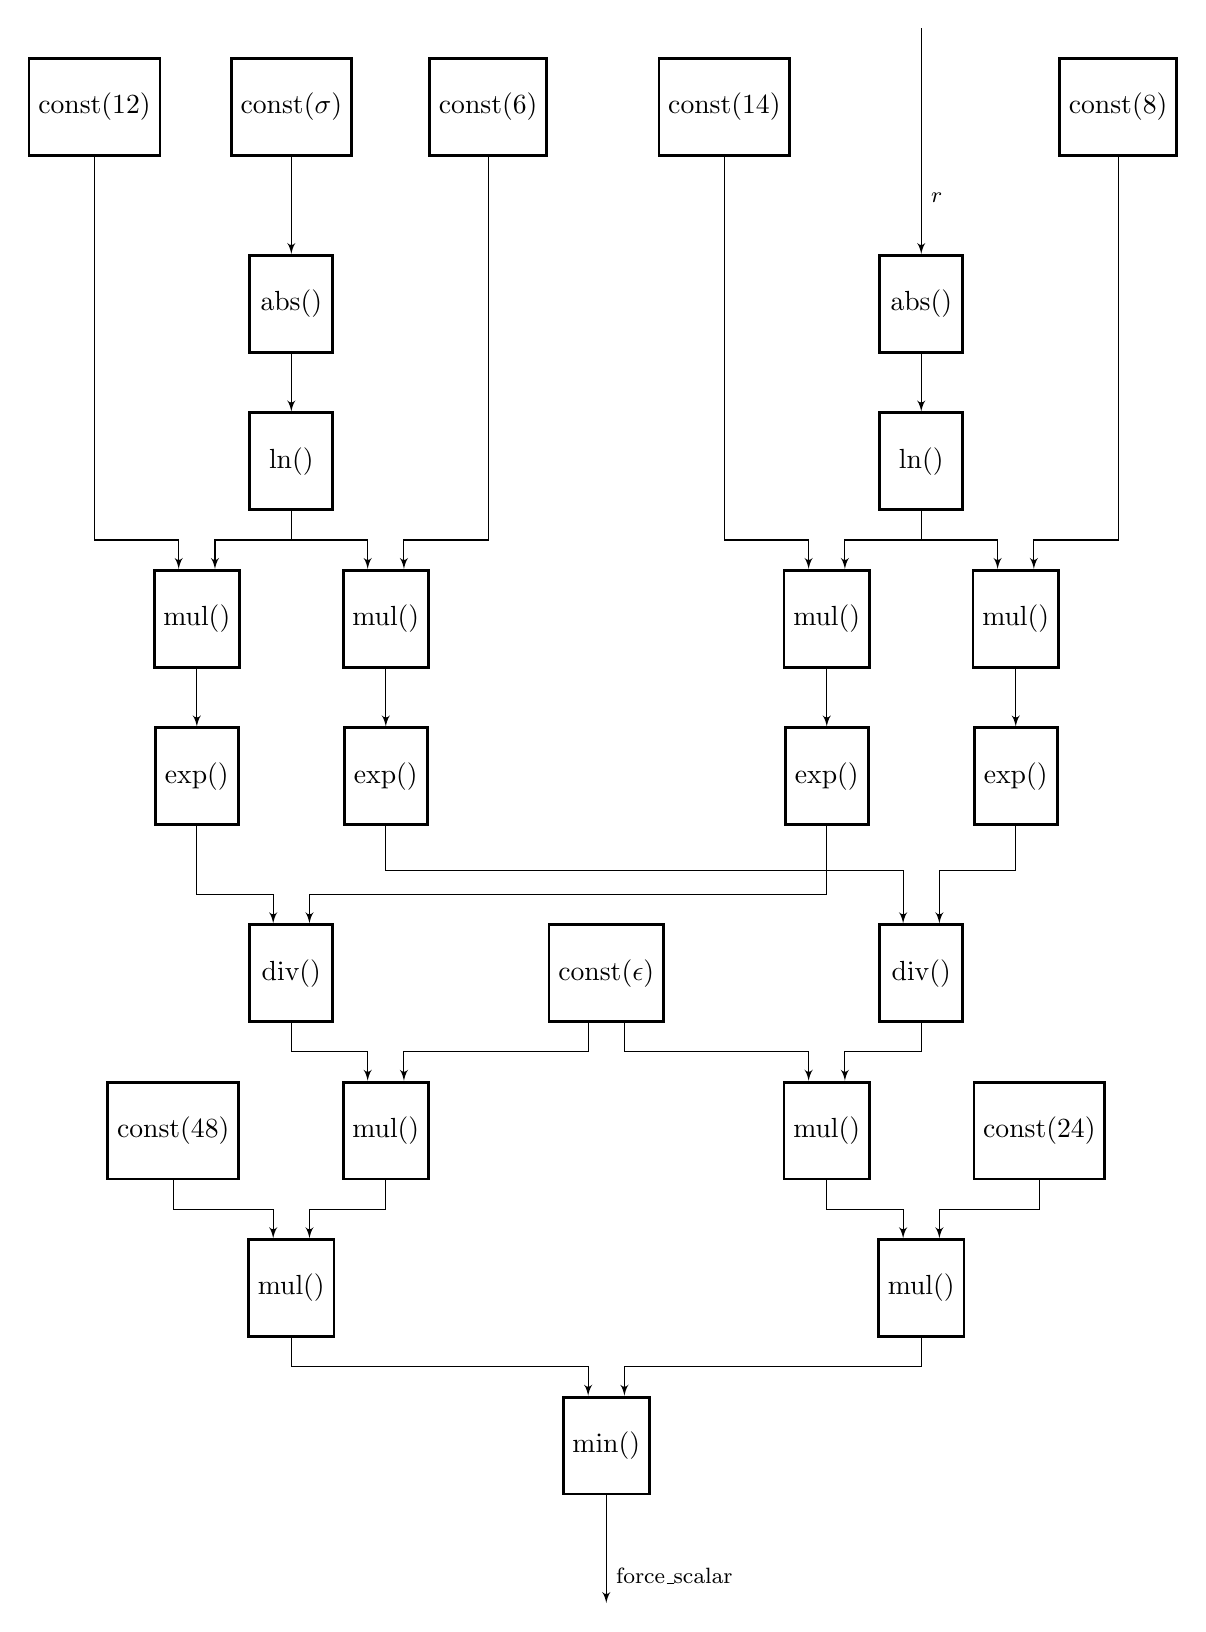
\begin{tikzpicture}

            \node[process] (twelve) at (-6.5,0) {const(12)};
            \node[process] (six) at (-1.5,0) {const(6)};
            \node[process] (sigma) at (-4,0) {const($\sigma$)};
            \node[process] (abs_sigma) at (-4,-2.5) {abs()};
            \node[process] (ln_sigma) at (-4,-4.5) {ln()};

            \node[process] (fourteen) at (1.5,0) {const(14)};
            \node[process] (eight) at (6.5,0) {const(8)};
            \node[process] (abs_r) at (4,-2.5) {abs()};
            \node[process] (ln_r) at (4,-4.5) {ln()};


            \node[process] (mul_12) at (-5.2,-6.5) {mul()};
            \node[process] (mul_6) at (-2.8,-6.5) {mul()};

            \node[process] (mul_14) at (2.8,-6.5) {mul()};
            \node[process] (mul_8) at (5.2,-6.5) {mul()};

            \node[process] (exp_12) at (-5.2,-8.5) {exp()};
            \node[process] (exp_6) at (-2.8,-8.5) {exp()};

            \node[process] (exp_14) at (2.8,-8.5) {exp()};
            \node[process] (exp_8) at (5.2,-8.5) {exp()};
            
            \node[process] (div_12_14) at (-4,-11) {div()};
            \node[process] (div_6_8) at (4,-11) {div()};

            \node[process] (epsilon) at (0,-11) {const($\epsilon$)};

            \node[process] (mul_12_14_eps) at (-2.8,-13) {mul()};
            \node[process] (mul_6_8_eps) at (2.8,-13) {mul()};

            \node[process] (fortyeight) at (-5.5,-13) {const(48)};
            \node[process] (twentyfour) at (5.5,-13) {const(24)};

            \node[process] (mul_48) at (-4,-15) {mul()};
            \node[process] (mul_24) at (4,-15) {mul()};

            \node[process] (min) at (0,-17) {min()};
            

            \path[draw, ->] (sigma.270) -- (abs_sigma.90);
            \path[draw, ->] (4,1) -- (abs_r.90) node [near end] {\footnotesize $r$};

            \path[draw, ->] (abs_sigma.270) -- (ln_sigma.90);
            \path[draw, ->] (abs_r.270) -- (ln_r.90);


            \path[draw, ->] (twelve.270) |- (-5.5, -5.5) -| (mul_12.110);
            \path[draw, ->] (ln_sigma.270) |- (-4.5, -5.5) -| (mul_12.70);
            
            \path[draw, ->] (six.270) |- (-2, -5.5) -| (mul_6.70);
            \path[draw, ->] (ln_sigma.270) |- (-3.5, -5.5) -| (mul_6.110);

            \path[draw, ->] (fourteen.270) |- (2, -5.5) -| (mul_14.110);
            \path[draw, ->] (ln_r.270) |- (3.5, -5.5) -| (mul_14.70);
            
            \path[draw, ->] (eight.270) |- (5.5, -5.5) -| (mul_8.70);
            \path[draw, ->] (ln_r.270) |- (4.5, -5.5) -| (mul_8.110);

            \path[draw, ->] (mul_12.270) -- (exp_12.90);
            \path[draw, ->] (mul_6.270) -- (exp_6.90);

            \path[draw, ->] (mul_14.270) -- (exp_14.90);
            \path[draw, ->] (mul_8.270) -- (exp_8.90);

            \path[draw, ->] (exp_12.270) |- (-4.5, -10) -| (div_12_14.110);
            \path[draw, ->] (exp_14.270) |- (-3.5, -10) -| (div_12_14.70);

            \path[draw, ->] (exp_6.270) |- (3.5, -9.7) -| (div_6_8.110);
            \path[draw, ->] (exp_8.270) |- (4.5, -9.7) -| (div_6_8.70);

            \path[draw, ->] (div_12_14.270) |- (-3.5, -12) -| (mul_12_14_eps.110);
            \path[draw, ->] (epsilon.250) |- (-2.5, -12) -| (mul_12_14_eps.70);
            
            \path[draw, ->] (div_6_8.270) |- (3.5, -12) -| (mul_6_8_eps.70);
            \path[draw, ->] (epsilon.290) |- (2.5, -12) -| (mul_6_8_eps.110);

            \path[draw, ->] (fortyeight.270) |- (-4.5, -14) -| (mul_48.110);
            \path[draw, ->] (mul_12_14_eps.270) |- (-3.5, -14) -| (mul_48.70);

            \path[draw, ->] (twentyfour.270) |- (4.5, -14) -| (mul_24.70);
            \path[draw, ->] (mul_6_8_eps.270) |- (3.5, -14) -| (mul_24.110);

            \path[draw, ->] (mul_48.270) |- (-3.5, -16) -| (min.110);
            \path[draw, ->] (mul_24.270) |- (2.5, -16) -| (min.70);

            \path[draw, ->] (min.270) -- (0,-19) node [near end] {\footnotesize force\_scalar};


            % \path[draw, ->] (testsim.282) -- (cache.80) node [near end] {\footnotesize ready};
            % \path[draw, ->] (cache.10) -| node [near start] {\footnotesize data array/i} (accram.260) node [near end] {\footnotesize \texttt{A}};
            % \path[draw, ->, red] (accram.280) |- node [pos=0.2] {\footnotesize \texttt{A}} (cache.350) node [near end] {\footnotesize data array};
            % \path[draw, ->] (testsim.5) -| node [near start] {\footnotesize i} (accram.80) node [near end] {\footnotesize \texttt{B}};
            % \path[draw, ->, red] (accram.100) |- node [pos=0.32] {\footnotesize \texttt{B}} (testsim.355) node [near end] {\footnotesize data};

            % \path[draw, ->] (cache.180) -| (-2.5,-3) |- (testsim.180) node [midway] {\footnotesize finished};

        \end{tikzpicture}
    }
    \caption{Force wrapper}
\end{figure}

\end{document}
